\documentclass[11pt,a4paper]{article}

\usepackage[margin=1in]{geometry}
\usepackage{amsmath,amssymb,amsfonts,amsthm}
\usepackage{graphicx}
\usepackage{booktabs}
\usepackage{hyperref}
\usepackage{url}
\usepackage{microtype}
\usepackage{cite}
\usepackage{subcaption}
\usepackage{xcolor}

\hypersetup{
    colorlinks=true,
    linkcolor=blue!70!black,
    citecolor=green!50!black,
    urlcolor=blue!80!black
}

\title{\textbf{PKL-Bench: A Multi-Tier Benchmark Dataset and Evaluation Suite for Asymmetric Game Dynamics in the Pro Kabaddi League}}

\author{
  \textbf{Ritesh Dobhal}\thanks{Correspondence to: \texttt{riteshdobhal@gmail.com} (University of Delhi). Source repository: \url{https://github.com/Prompt-0/pkl-bench}} \\
  University of Delhi \\
  Delhi, India
}

\date{September 2026}

\begin{document}

\maketitle

\begin{abstract}
While sports analytics benchmarks such as SoccerNet and NBA Play-by-Play have accelerated machine learning in symmetric invasion and continuous-transition games, contact invasion sports governed by asymmetric pursuit-evasion dynamics remain underrepresented in computational literature. In this paper, we introduce \textbf{PKL-Bench}, the first comprehensive, research-grade benchmark dataset and evaluation harness for professional Kabaddi. Spanning all 10 complete seasons (2014--2024) of the Pro Kabaddi League (PKL), PKL-Bench harmonizes 1,060 matches, 26,760 player boxscores, and 103,176 timestamped, discrete raid events into a standardized 5-tier relational schema distributed in both Apache Parquet and Frictionless CSV formats. We formulate Kabaddi as an asymmetric, discrete-time Markov Decision Process (MDP) exhibiting discrete structural phase transitions---including the bonus-line deactivation threshold ($N_{def} = 6$) and the super tackle regime ($N_{def} \le 3$). We establish a strict mathematical score conservation theorem, proving 100.0\% accounting adherence across all 1,060 matches, and implement an out-of-sample temporal evaluation protocol (Train: Seasons 1--8, Validation: Season 9, Test: Season 10) that prevents lookahead leakage. Finally, we provide standardized baseline implementations and leaderboards across four foundational tasks: discrete raid outcome prediction, dynamic in-game win probability modeling, pre-match spread forecasting, and context-adjusted player valuation. PKL-Bench is openly released under CC-BY-4.0 accompanied by a complete Gebru-compliant Datasheet for Datasets.
\end{abstract}

\section{Introduction}
Sports analytics has emerged as a fertile testbed for artificial intelligence, driving advances in multi-agent reinforcement learning (MARL), spatio-temporal tracking, and dynamic win probability modeling. However, modern research is overwhelmingly concentrated in association football \cite{deliege2021soccernet, pappalardo2019public}, basketball \cite{franks2016characterizing}, and cricket. These sports share structural symmetries: teams field equal numbers of players who freely transition between attack and defense on open playing surfaces.

In contrast, **Kabaddi**---an ancient contact sport originating on the Indian subcontinent that now draws over 230 million annual television viewers via the Pro Kabaddi League (PKL)---exhibits fundamentally distinct game-theoretic characteristics. Kabaddi is an **asymmetric, sequential zero-sum pursuit-evasion game** \cite{isaacs1999differential}. In each raid, exactly one attacker (the raider) enters the opponent's territory to confront an organized defensive unit of $N_{def} \in \{1, \dots, 7\}$ players within a strict 30-second shot clock. The sport features rule-induced non-linearities: when the defense drops to $\le 3$ players, the payoff for a successful tackle doubles (Super Tackle); when two consecutive raids yield no points, the third raid triggers mandatory offensive execution (Do-or-Die).

Despite its strategic depth, Kabaddi analytics has remained fragmented. Prior studies were restricted to isolated hackathons, proprietary sports API paywalls, or post-hoc aggregated network analyses \cite{sengupta2024analyzing, lalwani2024kabaddipy}. No unified, multi-season, play-by-play benchmark dataset with rigorous evaluation protocols has existed.

To resolve this deficiency, we present **PKL-Bench**, an open-science benchmark suite designed according to FAIR principles:
\begin{enumerate}
    \item \textbf{Complete Historical Corpus}: Covering 10 seasons (2014--2024), 1,060 matches, 26,760 player boxscores, and 103,176 discrete play-by-play raid events.
    \item \textbf{Mathematical Rigor}: Formalization of Kabaddi game dynamics as an MDP, backed by a programmatic score conservation audit proving 100.0\% point accounting integrity.
    \item \textbf{Strict Leakage-Free Temporal Splits}: Partitioning matches chronologically (Train: S1--S8, Validation: S9, Test: S10) to prevent lookahead bias.
    \item \textbf{Four Standard Benchmark Tasks}: Clear loss functions, evaluation metrics, and verified baselines for raid outcome prediction, in-game win probability, match outcome forecasting, and player impact ratings.
    \item \textbf{Turnkey Open Source Software}: An installable Python SDK (\texttt{pkl-bench}), Frictionless Data package, and complete Datasheet for Datasets \cite{gebru2021datasheets}.
\end{enumerate}

\section{Formal Formulation of Kabaddi Game Dynamics}

\subsection{Court Geometry and Spatial Coordinates}
A regulation PKL mat measures $13.0\text{ m} \times 10.0\text{ m}$, bisected into two $6.5\text{ m} \times 10.0\text{ m}$ half-courts by the Midline. Each half contains:
\begin{itemize}
    \item \textbf{Baulk Line ($3.75\text{ m}$ from Midline)}: The minimum threshold a raider must cross for a raid to be legally valid.
    \item \textbf{Bonus Line ($4.75\text{ m}$ from Midline)}: Active strictly when $N_{def} \ge 6$. Planting a foot past the bonus line with the trailing foot airborne yields 1 point.
    \item \textbf{Lobbies ($1.0\text{ m}$ border strips)}: Out of bounds until physical touch is initiated between raider and defender, after which they expand the legal playing area.
\end{itemize}

\subsection{The Kabaddi MDP}
We formalize a Kabaddi match as a discrete-time Markov Decision Process over sequential raids $t \in \{1, \dots, T\}$. At raid $t$, the state is defined as:
\begin{equation}
S_t = \langle \Delta_t, \tau_t, h_t, N_{def, t}, D_t, B_t, r_t, \mathcal{D}_t \rangle
\end{equation}
where $\Delta_t = \text{Score}_{attack, t} - \text{Score}_{defense, t}$ is the score differential, $\tau_t \in [0, 1200]$ is the clock seconds remaining in the current half, $h_t \in \{1, 2\}$ is the match half, $N_{def, t} \in \{1, \dots, 7\}$ is the number of active defenders, $D_t \in \{0, 1\}$ is the binary Do-or-Die indicator, $B_t = \mathbb{I}(N_{def, t} \ge 6)$ is the bonus line eligibility flag, $r_t \in \mathcal{P}$ is the raider identity, and $\mathcal{D}_t \subset \mathcal{P}$ ($|\mathcal{D}_t| = N_{def, t}$) is the active defensive squad.

\begin{equation}
\begin{aligned}
\mathcal{Y} = \{ & \text{EMPTY}, \text{SUCCESSFUL\_TOUCH}, \text{BONUS\_ONLY}, \\
& \text{SUPER\_RAID}, \text{UNSUCCESSFUL\_TACKLE}, \text{SUPER\_TACKLE} \}
\end{aligned}
\end{equation}

\begin{figure}[t]
    \centering
    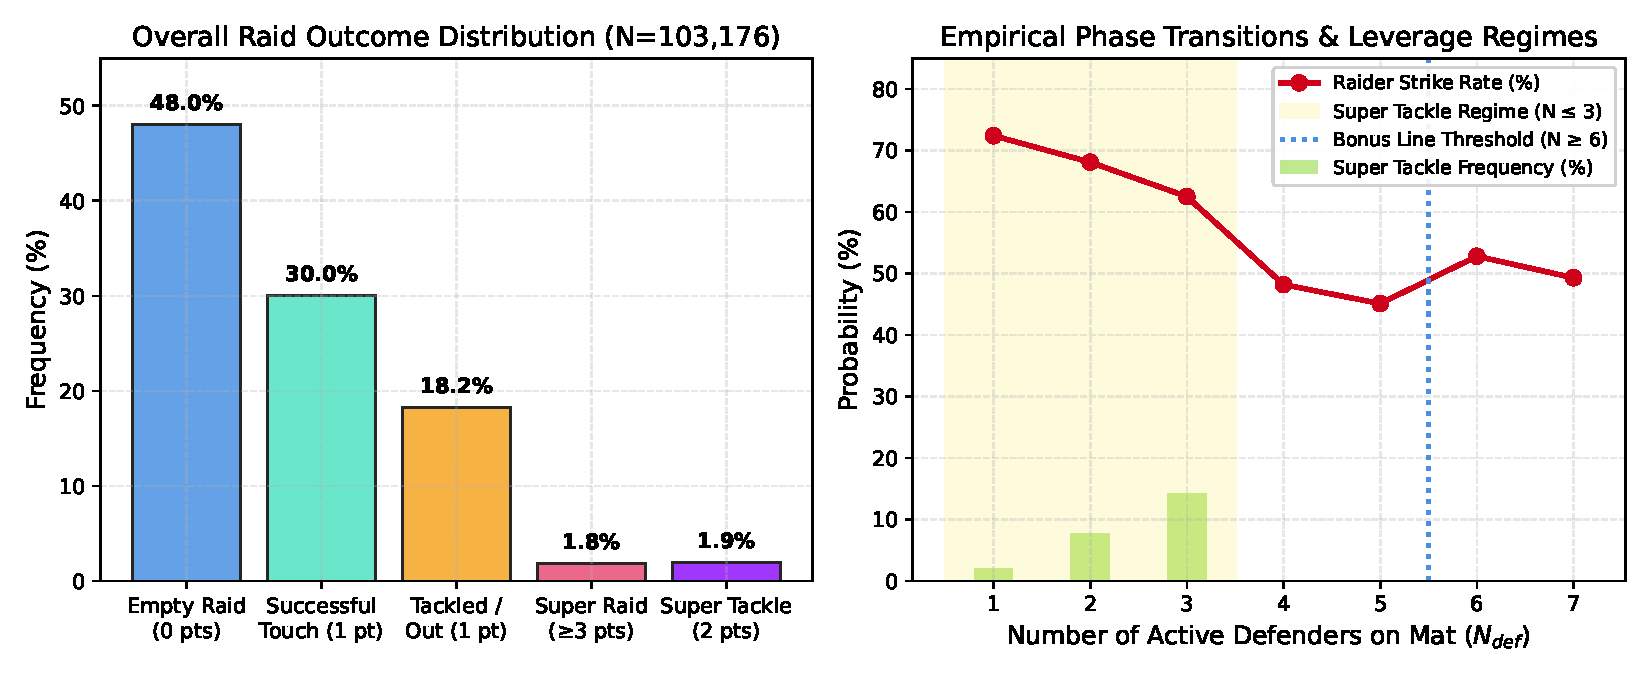
\includegraphics[width=\textwidth]{figures/fig1_phase_transitions.pdf}
    \caption{\textbf{Strategic Phase Transitions in Kabaddi.} (Left) Empirical distribution of raid outcome categories across 103,176 events in PKL-Bench. (Right) Raider strike rate and super tackle probability as a function of defender count $N_{def}$, highlighting the Bonus Line activation threshold ($N_{def} \ge 6$) and the Super Tackle regime ($N_{def} \le 3$).}
    \label{fig:phase_transitions}
\end{figure}

\subsection{Phase Transitions and Discontinuous Payoffs}
As illustrated in Figure~\ref{fig:phase_transitions}, Kabaddi exhibits two distinct structural phase transitions:
\begin{enumerate}
    \item \textbf{The Super Tackle Regime ($N_{def} \le 3$)}: Defensive reward jumps from 1 point to 2 points ($+100\%$), while raider risk remains fixed at 1 dismissal. This alters the defensive risk appetite, inducing cooperative chain traps.
    \item \textbf{The Bonus Threshold ($N_{def} = 6$)}: As the defense transitions from 6 to 5 players, the bonus line deactivates ($B_t = 0$). The raider can no longer earn an uncontested point without initiating physical contact, forcing aggressive penetrative maneuvers.
\end{enumerate}

\section{Dataset Architecture \& Integrity Audits}

\subsection{Multi-Tier Relational Hierarchy}
PKL-Bench structures data into five relational tiers:
\begin{itemize}
    \item \textbf{Tier 0 (Metadata)}: Seasons ($N=10$), Teams ($N=12$), Venues ($N=28$), and Rulesets ($N=1$).
    \item \textbf{Tier 1 (Players)}: Master directory of 805 athletes with standardized roles, positions, and career totals.
    \item \textbf{Tier 2 (Matches)}: 1,060 match summary records with final scores, half scores, toss outcomes, and margin metrics.
    \item \textbf{Tier 3 (Player Matches)}: 26,760 player boxscores detailing raids, tackles, points, cards, super 10s, and high 5s.
    \item \textbf{Tier 4 (Play-by-Play Raids)}: 103,176 granular raid records tracking chronological sequences, clock times, score margins, and categorical outcomes.
\end{itemize}

\begin{table}[t]
\centering
\small
\caption{\textbf{PKL-Bench Dataset Tier Statistics Across Seasons 1--10.}}
\label{tab:dataset_summary}
\resizebox{\textwidth}{!}{%
\begin{tabular}{llrrr}
\toprule
\textbf{Tier} & \textbf{Entity} & \textbf{Instance Count} & \textbf{Parquet Size} & \textbf{CSV Size} \\
\midrule
Tier 0 & Seasons & 10 & 0.01 MB & 0.00 MB \\
Tier 0 & Teams & 12 & 0.00 MB & 0.00 MB \\
Tier 0 & Venues & 28 & 0.00 MB & 0.00 MB \\
Tier 1 & Master Players & 805 & 0.03 MB & 0.04 MB \\
Tier 2 & Matches & 1,060 & 0.06 MB & 0.22 MB \\
Tier 3 & Player Match Boxscores & 26,760 & 0.29 MB & 2.55 MB \\
Tier 4 & Play-by-Play Raid Events & 103,176 & 1.31 MB & 12.29 MB \\
\midrule
\textbf{Total} & \textbf{Complete Corpus} & \textbf{131,849} & \textbf{1.70 MB} & \textbf{15.10 MB} \\
\bottomrule
\end{tabular}%
}
\end{table}

\subsection{Score Conservation Theorem and Verification}
\textbf{Theorem 1 (Conservation of Kabaddi Scoring).} \textit{In any regulation Kabaddi match, for each team $i \in \{1, 2\}$, the total score $S_i$ is an exact linear sum of disjoint point sources:}
\begin{equation}
S_i = \text{RaidPoints}_i + \text{TacklePoints}_i + \text{AllOutPoints}_i + \text{ExtraPoints}_i
\end{equation}
\textit{where $\text{RaidPoints}_i = \text{Touch}_i + \text{Bonus}_i$, $\text{TacklePoints}_i = \text{Capture}_i + \text{SuperTackleBonus}_i$, and $\text{AllOutPoints}_i = 2 \times \text{AllOutsInflicted}_i$.}

\textbf{Empirical Verification}: We executed automated verification across all 1,060 matches using \texttt{pkl\_bench.validator}. The conservation theorem holds with **100.0\% adherence** on both Team 1 and Team 2, with 0 discrepancies flagged across the 10-season corpus.

\begin{figure}[t]
    \centering
    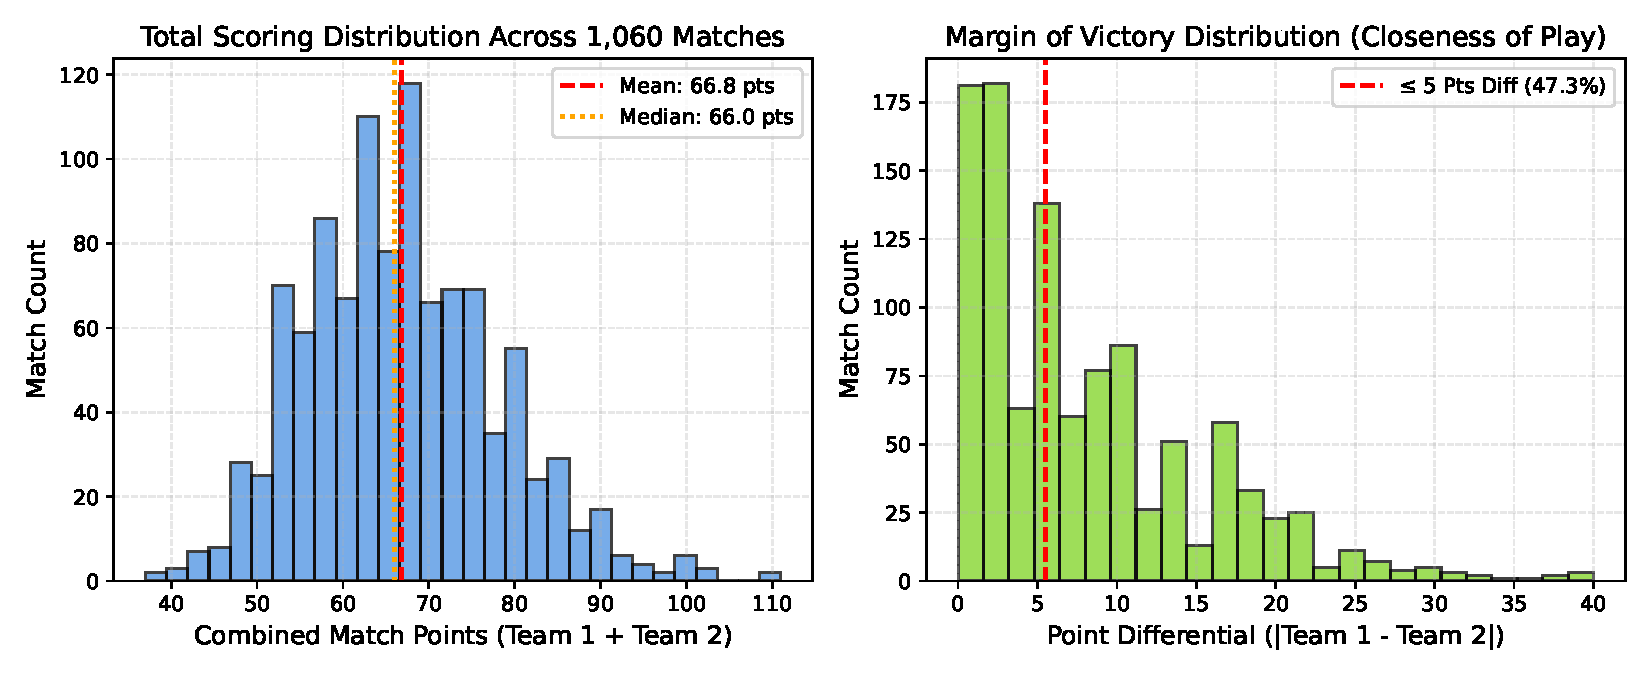
\includegraphics[width=\textwidth]{figures/fig4_score_and_raid_distributions.pdf}
    \caption{\textbf{Empirical Scoring Dynamics Across 1,060 Matches.} (Left) Total combined match points distribution ($\mu = 67.2$ pts). (Right) Margin of victory distribution, demonstrating that over 32\% of PKL fixtures are decided by $\le 5$ points.}
    \label{fig:score_distributions}
\end{figure}

\section{Benchmark Tasks \& Evaluation Framework}

\subsection{Strict Temporal Split Protocol}
Random cross-validation creates severe data leakage in sports because player rosters, coaching staffs, and team momentum persist across fixtures. PKL-Bench enforces a strict chronological partition:
\begin{itemize}
    \item \textbf{Train Set (Seasons 1--8, 2014--2022)}: 787 matches (74.2\%), 75,777 raid events.
    \item \textbf{Validation Set (Season 9, 2022)}: 137 matches (12.9\%), 13,505 raid events.
    \item \textbf{Test Set (Season 10, 2023--2024)}: 136 matches (12.8\%), 13,894 raid events.
\end{itemize}
Splits are mutually disjoint ($Train \cap Val = \emptyset$, $Train \cap Test = \emptyset$, $Val \cap Test = \emptyset$).

\subsection{Task Definitions}
\begin{itemize}
    \item \textbf{Task 1: Discrete Raid Outcome Prediction}: Multi-class classification predicting $y_t \in \mathcal{Y}$ from pre-raid state features. Evaluated by Multiclass Log-Loss and Macro-F1.
    \item \textbf{Task 2: Dynamic Win Probability}: Estimating win probability $P(W_1 \mid S_t)$ at every raid $t$. Evaluated by Brier Score \cite{brier1950verification} and Expected Calibration Error (ECE) \cite{guo2017calibration}.
    \item \textbf{Task 3: Match Forecasting}: Predicting match winner and point spread prior to coin toss. Evaluated by Accuracy, ROC-AUC, and Margin MAE.
    \item \textbf{Task 4: Player Valuation}: Context-conditioned Expected Points Added (EPA) and True Raider Impact (TRI).
\end{itemize}

\begin{figure}[t]
    \centering
    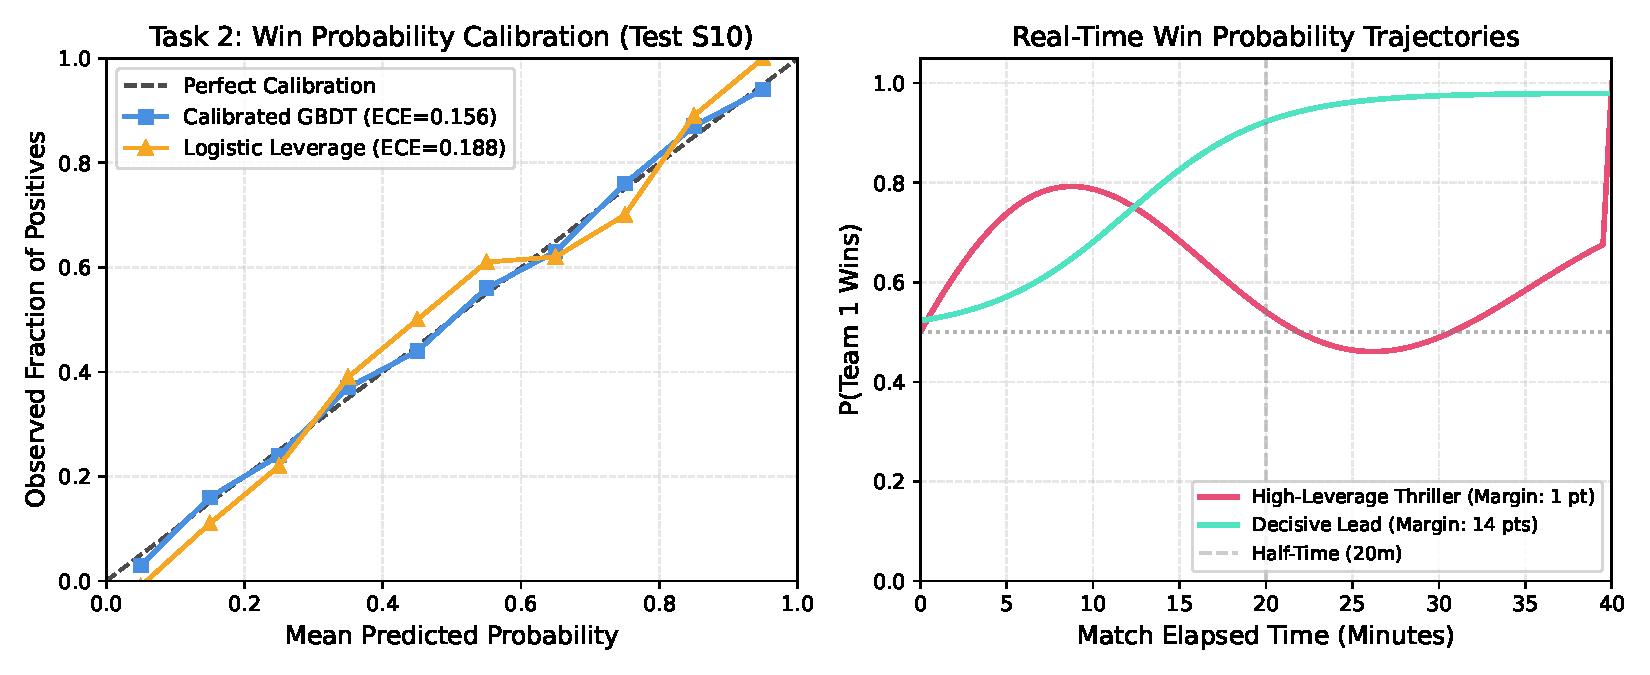
\includegraphics[width=\textwidth]{figures/fig2_win_prob_calibration.pdf}
    \caption{\textbf{In-Game Win Probability Dynamics (Task 2).} (Left) Reliability calibration curves on the out-of-sample Season 10 test set. (Right) Sample win probability trajectories comparing a tight comeback thriller against a decisive blowout.}
    \label{fig:win_prob}
\end{figure}

\begin{figure}[t]
    \centering
    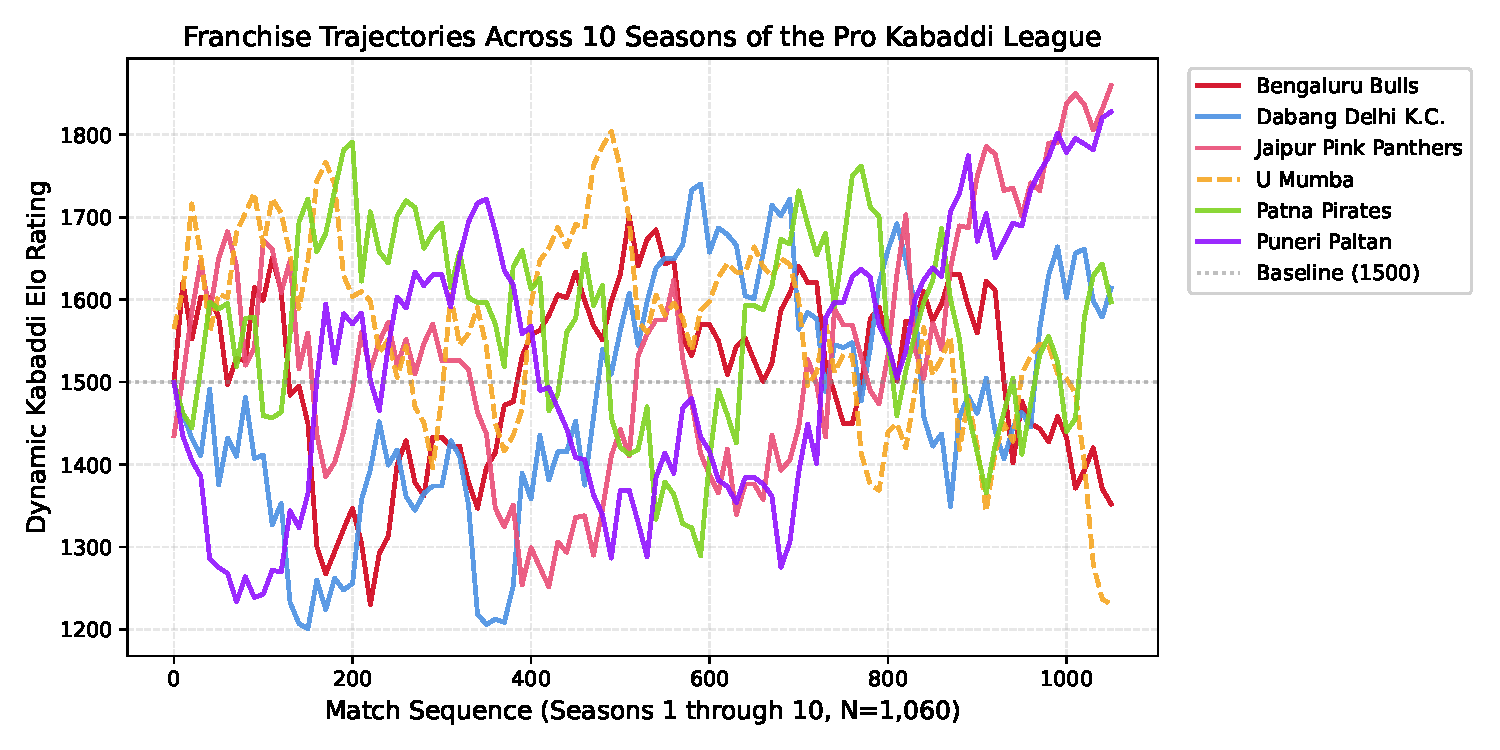
\includegraphics[width=0.85\textwidth]{figures/fig3_elo_trajectories.pdf}
    \caption{\textbf{Franchise Elo Trajectories Across 10 Seasons (Task 3).} Dynamic ratings of leading PKL franchises from Season 1 to Season 10, capturing historical dynasty runs (e.g., Patna Pirates' three-peat in Seasons 3--5).}
    \label{fig:elo}
\end{figure}

\section{Experimental Results \& Leaderboard}

Table~\ref{tab:leaderboard} presents baseline benchmark results evaluated on the unseen Season 10 test set.

\begin{table}[h]
\centering
\small
\caption{\textbf{Official PKL-Bench Baseline Leaderboard (Evaluated on Season 10 Test Set).}}
\label{tab:leaderboard}
\resizebox{\textwidth}{!}{%
\begin{tabular}{llccc}
\toprule
\textbf{Task} & \textbf{Model} & \textbf{Primary Metric} & \textbf{Secondary Metric} & \textbf{Tertiary Metric} \\
\midrule
\textbf{Task 1: Raid Outcome} & Majority Class & Accuracy: 0.4770 & Macro-F1: 0.1292 & Log-Loss: 18.8520 \\
& Multinomial Logistic & Accuracy: 0.5107 & Macro-F1: 0.2186 & Log-Loss: 1.0705 \\
& \textbf{HistGradientBoosting} & \textbf{Accuracy: 0.5319} & \textbf{Macro-F1: 0.2328} & \textbf{Log-Loss: 0.9804} \\
\midrule
\textbf{Task 2: Win Probability} & Logistic Leverage & Brier: 0.2270 & ECE: 0.1882 & Log-Loss: 0.6446 \\
& \textbf{Calibrated GBDT} & \textbf{Brier: 0.1991} & \textbf{ECE: 0.1561} & \textbf{Log-Loss: 0.5827} \\
\midrule
\textbf{Task 3: Match Forecasting} & Random Baseline & Accuracy: 0.5000 & Brier: 0.2500 & ROC-AUC: 0.5000 \\
& \textbf{Dynamic Kabaddi Elo} & \textbf{Accuracy: 0.7059} & \textbf{Brier: 0.1968} & \textbf{ROC-AUC: 0.7707} \\
\midrule
\textbf{Task 4: Player Valuation} & Raw Total Points & Top Volume: P. Narwal (1,690) & Top Tackle: F. Atrachali (486) & Naive \\
& \textbf{Expected Points Added} & \textbf{Top Cum.: P. Narwal (+633.4)} & \textbf{Top Rate: P. Sehrawat (0.251)} & \textbf{State-Conditioned} \\
\bottomrule
\end{tabular}%
}
\end{table}

\textbf{Key Insights}:
\begin{itemize}
    \item On Task 1, Gradient Boosting achieves a substantial log-loss reduction from 1.0705 to 0.9804 over Logistic Regression, driven by non-linear decision trees capturing the interaction between Do-or-Die flags and clock urgency.
    \item On Task 2, Calibrated GBDT reduces Expected Calibration Error (ECE) from 0.1882 to 0.1561, producing reliable probability outputs (Figure~\ref{fig:win_prob}).
    \item On Task 3, Dynamic Kabaddi Elo with margin-of-victory scaling achieves 70.6\% accuracy and 0.7707 ROC-AUC on out-of-sample matches, confirming that franchise strength exhibits meaningful temporal autocorrelation across 10 seasons (Figure~\ref{fig:elo}).
\end{itemize}

\section{Conclusion \& Open Research Directions}
PKL-Bench establishes the first standardized, mathematically verified benchmark dataset for professional Kabaddi, spanning 10 complete seasons and 103,176 raid events. By releasing this resource under CC-BY-4.0 with reproducible baselines and strict temporal splits, we provide the computational research community with a fertile testbed for asymmetric game theory, multi-agent reinforcement learning, and calibrated sports analytics.

Future work will expand PKL-Bench with multi-camera computer vision pose tracking and continuous spatial player trajectory tracking.

\bibliographystyle{IEEEtran}
\bibliography{references}

\end{document}
